% No me parece necesaria la explicación (lo dice el título)
% A continuación se procede a explicar las pruebas realizadas en cada una de las áreas mencionadas anteriormente
\subsection{Pruebas en el diseño de las piezas 3D}
Desde los momentos iniciales del proceso de impresión se observa que ciertas partes de las piezas impresas no concuerdan en tamaño con lo especificado en el diseño 3D. Este problema se hace más evidente en piezas que requieren de alta precisión como pueden ser los agujeros para los tornillos o los dientes de los engranajes.

Dado que existe esta diferencia entre el tamaño real y el tamaño del diseño, durante el desarrollo se realizan varias pruebas para determinar qué tamaño es necesario definir en el diseño para que, al imprimir, se obtenga la medida deseada.

Estas pruebas se han tenido que hacer para determinar el diámetro necesario para los tornillos de métricas M3 y M4 junto con el de los ejes y los rodamientos.

Las pruebas han consistido principalmente en imprimir piezas con varios agujeros de distinto diámetro con el objetivo de averiguar cuál longitud es la adecuada.

% A continuación se pueden observar dichas piezas.
En la figura \ref{fig:diam_tests} se pueden ver distintas pruebas realizadas a tales
efectos:

\begin{figure}[H]
    \centering
    \begin{minipage}{.48\linewidth}
        \centering
        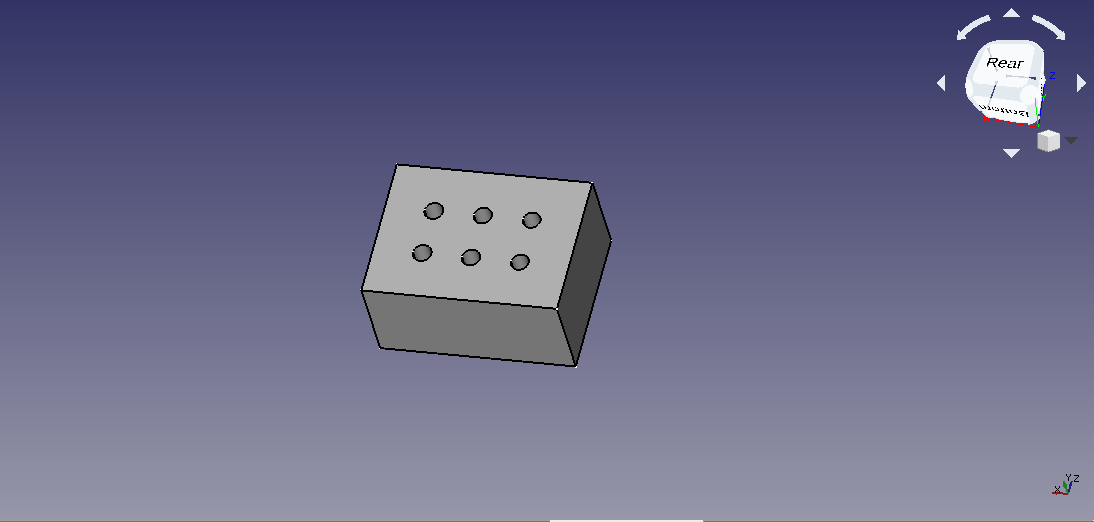
\includegraphics[width=\linewidth]{pictures/LadrilloPrueba.png}
        \caption{Pieza de prueba para tornillos M4.}
        \label{fig:prueba_m4}
    \end{minipage}
    \hfill
    \begin{minipage}{.48\linewidth}
        \centering
        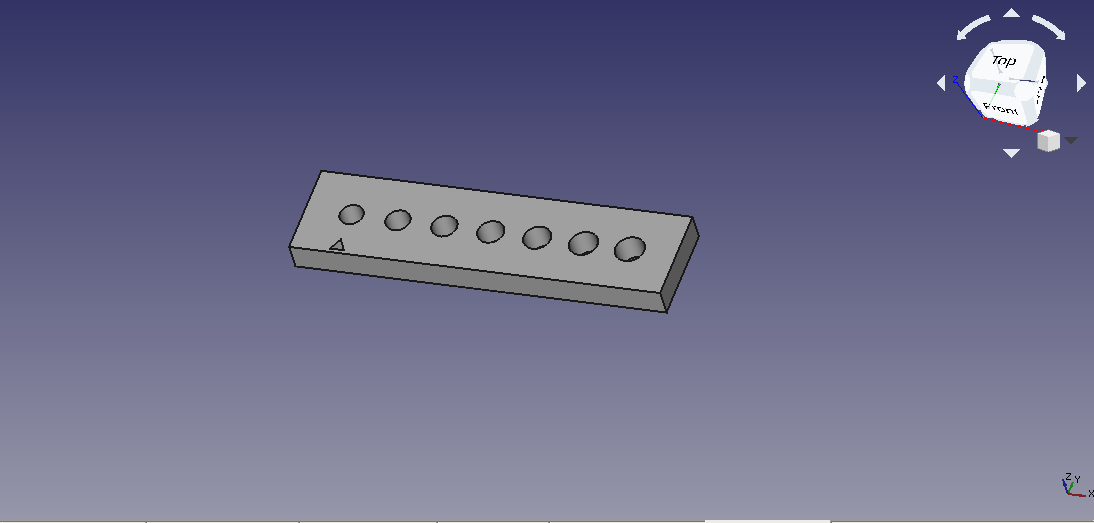
\includegraphics[width=\linewidth]{pictures/PruebaM3.png}
        \caption{Pieza de prueba para tornillos M3.}
        \label{fig:prueba_m3}
    \end{minipage}
    \\[1ex]
    \begin{minipage}{.7\linewidth}
        \centering
        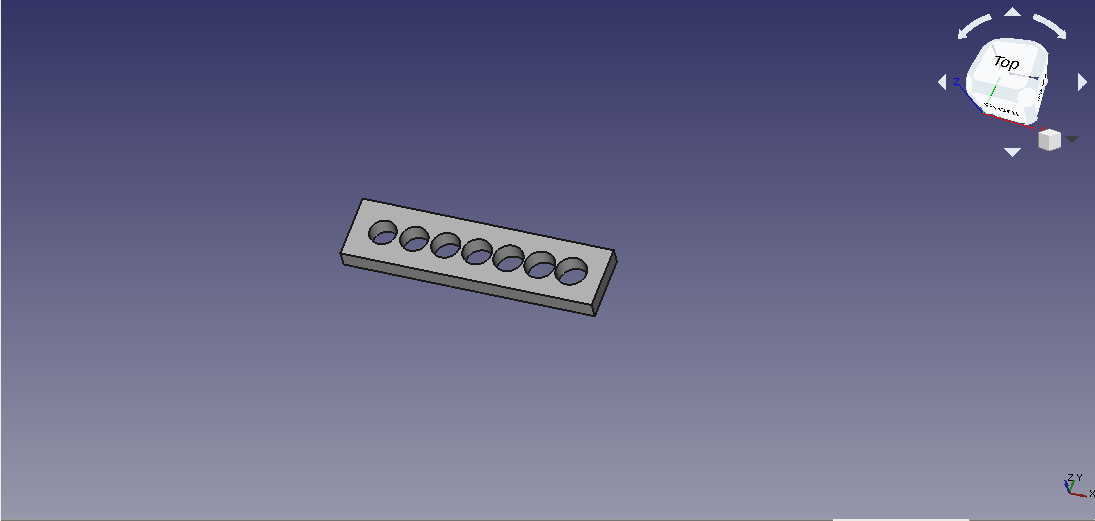
\includegraphics[width=\linewidth]{pictures/PruebaEje.png}
        \caption{Pieza de prueba para ejes de $\numprint[mm]{4}$ de diámetro.}
        \label{fig:prueba_eje}
    \end{minipage}
    \caption{Distintas pruebas realizadas para obtener el tamaño buscado para %
    métricas M3 y M4 así como los ejes de $\numprint[mm]{4}$ de diámetro.}
    \label{fig:diam_tests}
\end{figure}

% \begin{figure}[H]
%     \centering
%     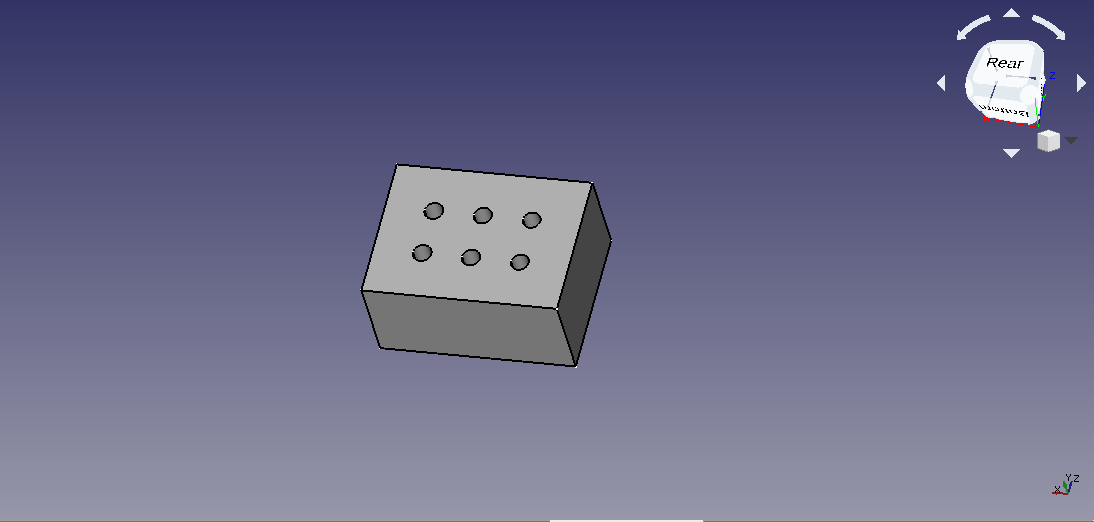
\includegraphics[width=.7\linewidth]{pictures/LadrilloPrueba.png}
%     \caption{Pieza de prueba para tornillos M4.}
%     \label{fig:prueba_m4}
% \end{figure}

% \begin{figure}[H]
%     \centering
%     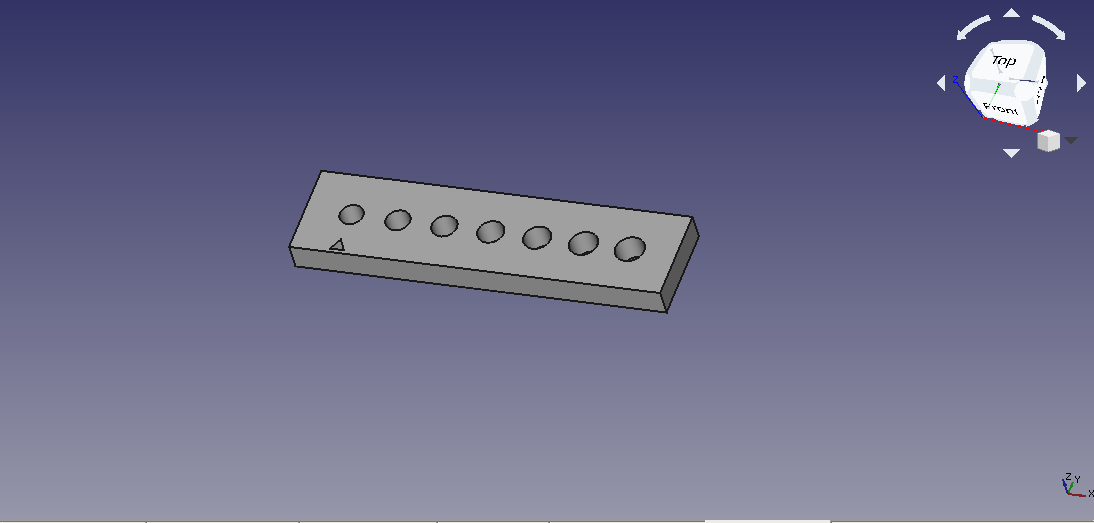
\includegraphics[width=.7\linewidth]{pictures/PruebaM3.png}
%     \caption{Pieza de prueba para tornillos M3.}
%     \label{fig:prueba_m3}
% \end{figure}

% \begin{figure}[H]
%     \centering
%     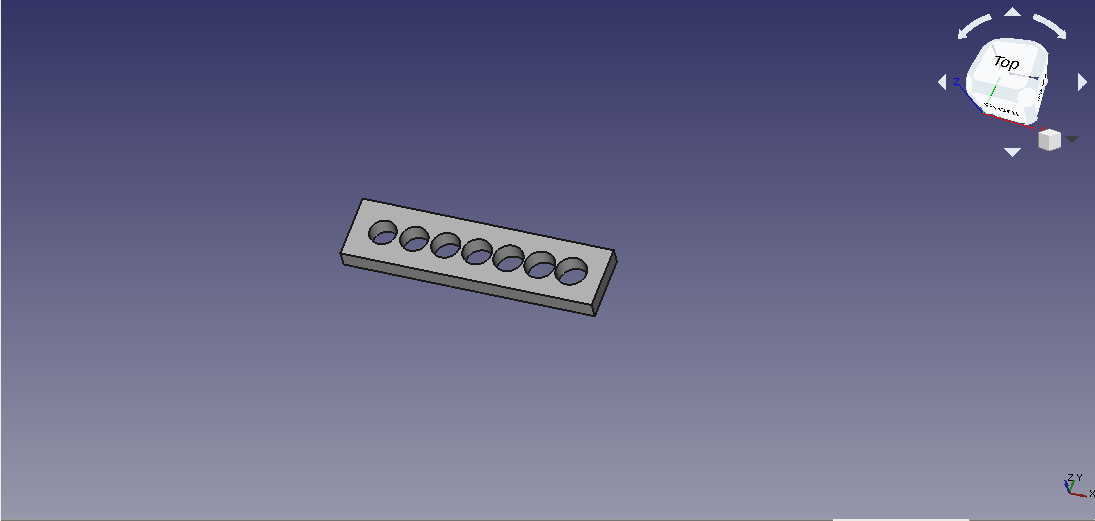
\includegraphics[width=.7\linewidth]{pictures/PruebaEje.png}
%     \caption{Pieza de prueba para eje de $\numprint[mm]{4}$ de diámetro.}
%     \label{fig:prueba_eje}
% \end{figure}

Tras realizar estas pruebas se tomaron las siguientes decisiones técnicas:

\begin{itemize}
    \item Para tornillos de métrica M3 (véase figura \ref{fig:prueba_m3}) el agujero del diseño 3D deberá tener $\numprint[mm]{2.8}$ de diámetro. Con esta longitud se consigue suficiente material adicional en las paredes del agujero para que, tras utilizar la herramienta de hacer machos, quede una rosca suficientemente profunda.

    Para diámetros menores, el macho no podía ser introducido en el agujero y por tanto no se podía hacer rosca mientras que, para diámetros mayores, el macho entraba con demasiada holgura o bien no había suficiente material adicional para crear una rosca resistente.
    
    Cabe recordar que los tornillos empleados son metálicos y que el agujero es sobre material plástico, por lo que una rosca resistente es necesaria debido al desgaste que el tornillo ejerce sobre la montura.
    \item Para tornillos de métrica M4 (véase figura \ref{fig:prueba_m4}) el agujero del diseño 3D deberá tener $\numprint[mm]{3.8}$ de diámetro. Las razones son las mismas que las expuestas anteriormente para el tornillo de métrica M3.
    \item En el caso de los ejes se siguió una metodología similar.
    Para un eje de $\numprint[mm]{4}$ de diámetro se debía dejar una agujero de entre $\numprint[mm]{3.9}$ y $\numprint[mm]{4.1}$ de diámetro dependiendo de la holgura que se desee.    
\end{itemize}

Por otro lado, se han tenido que hacer pruebas para determinar el módulo adecuado para el engranaje exterior que transmitiría el movimiento desde el eje motor hasta las piezas que se ensamblan con él.

\begin{figure}[H]
    \centering
    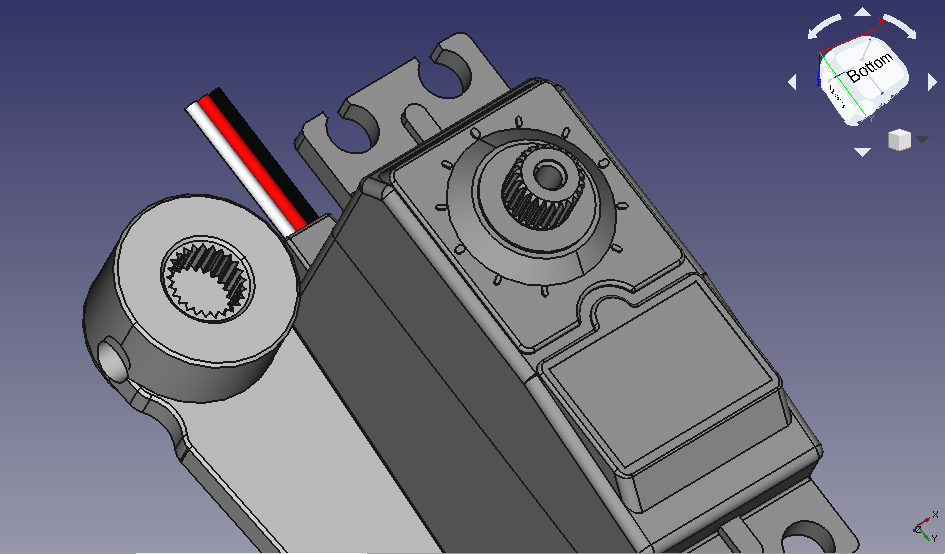
\includegraphics[width=.7\linewidth]{pictures/ComparativaEngranajes.png}
    \caption{Modelos 3D del motor empleado junto a una pieza que se ensambla en su eje.}
    \label{fig:comparativa_engranajes}
\end{figure}

Como se observa en la figura \ref{fig:comparativa_engranajes}, las piezas que van engranadas directamente en el eje han de tener un número determinado de dientes y un diámetro concreto.

La cantidad de dientes viene dada por el engranaje del motor (figura \ref{fig:motor_teeth_count}), el cual no puede ser modificado y es una restricción ajena al proceso de diseño. Sin embargo, se tuvieron que hacer pruebas para determinar el diámetro adecuado.

\begin{figure}[H]
    \centering
    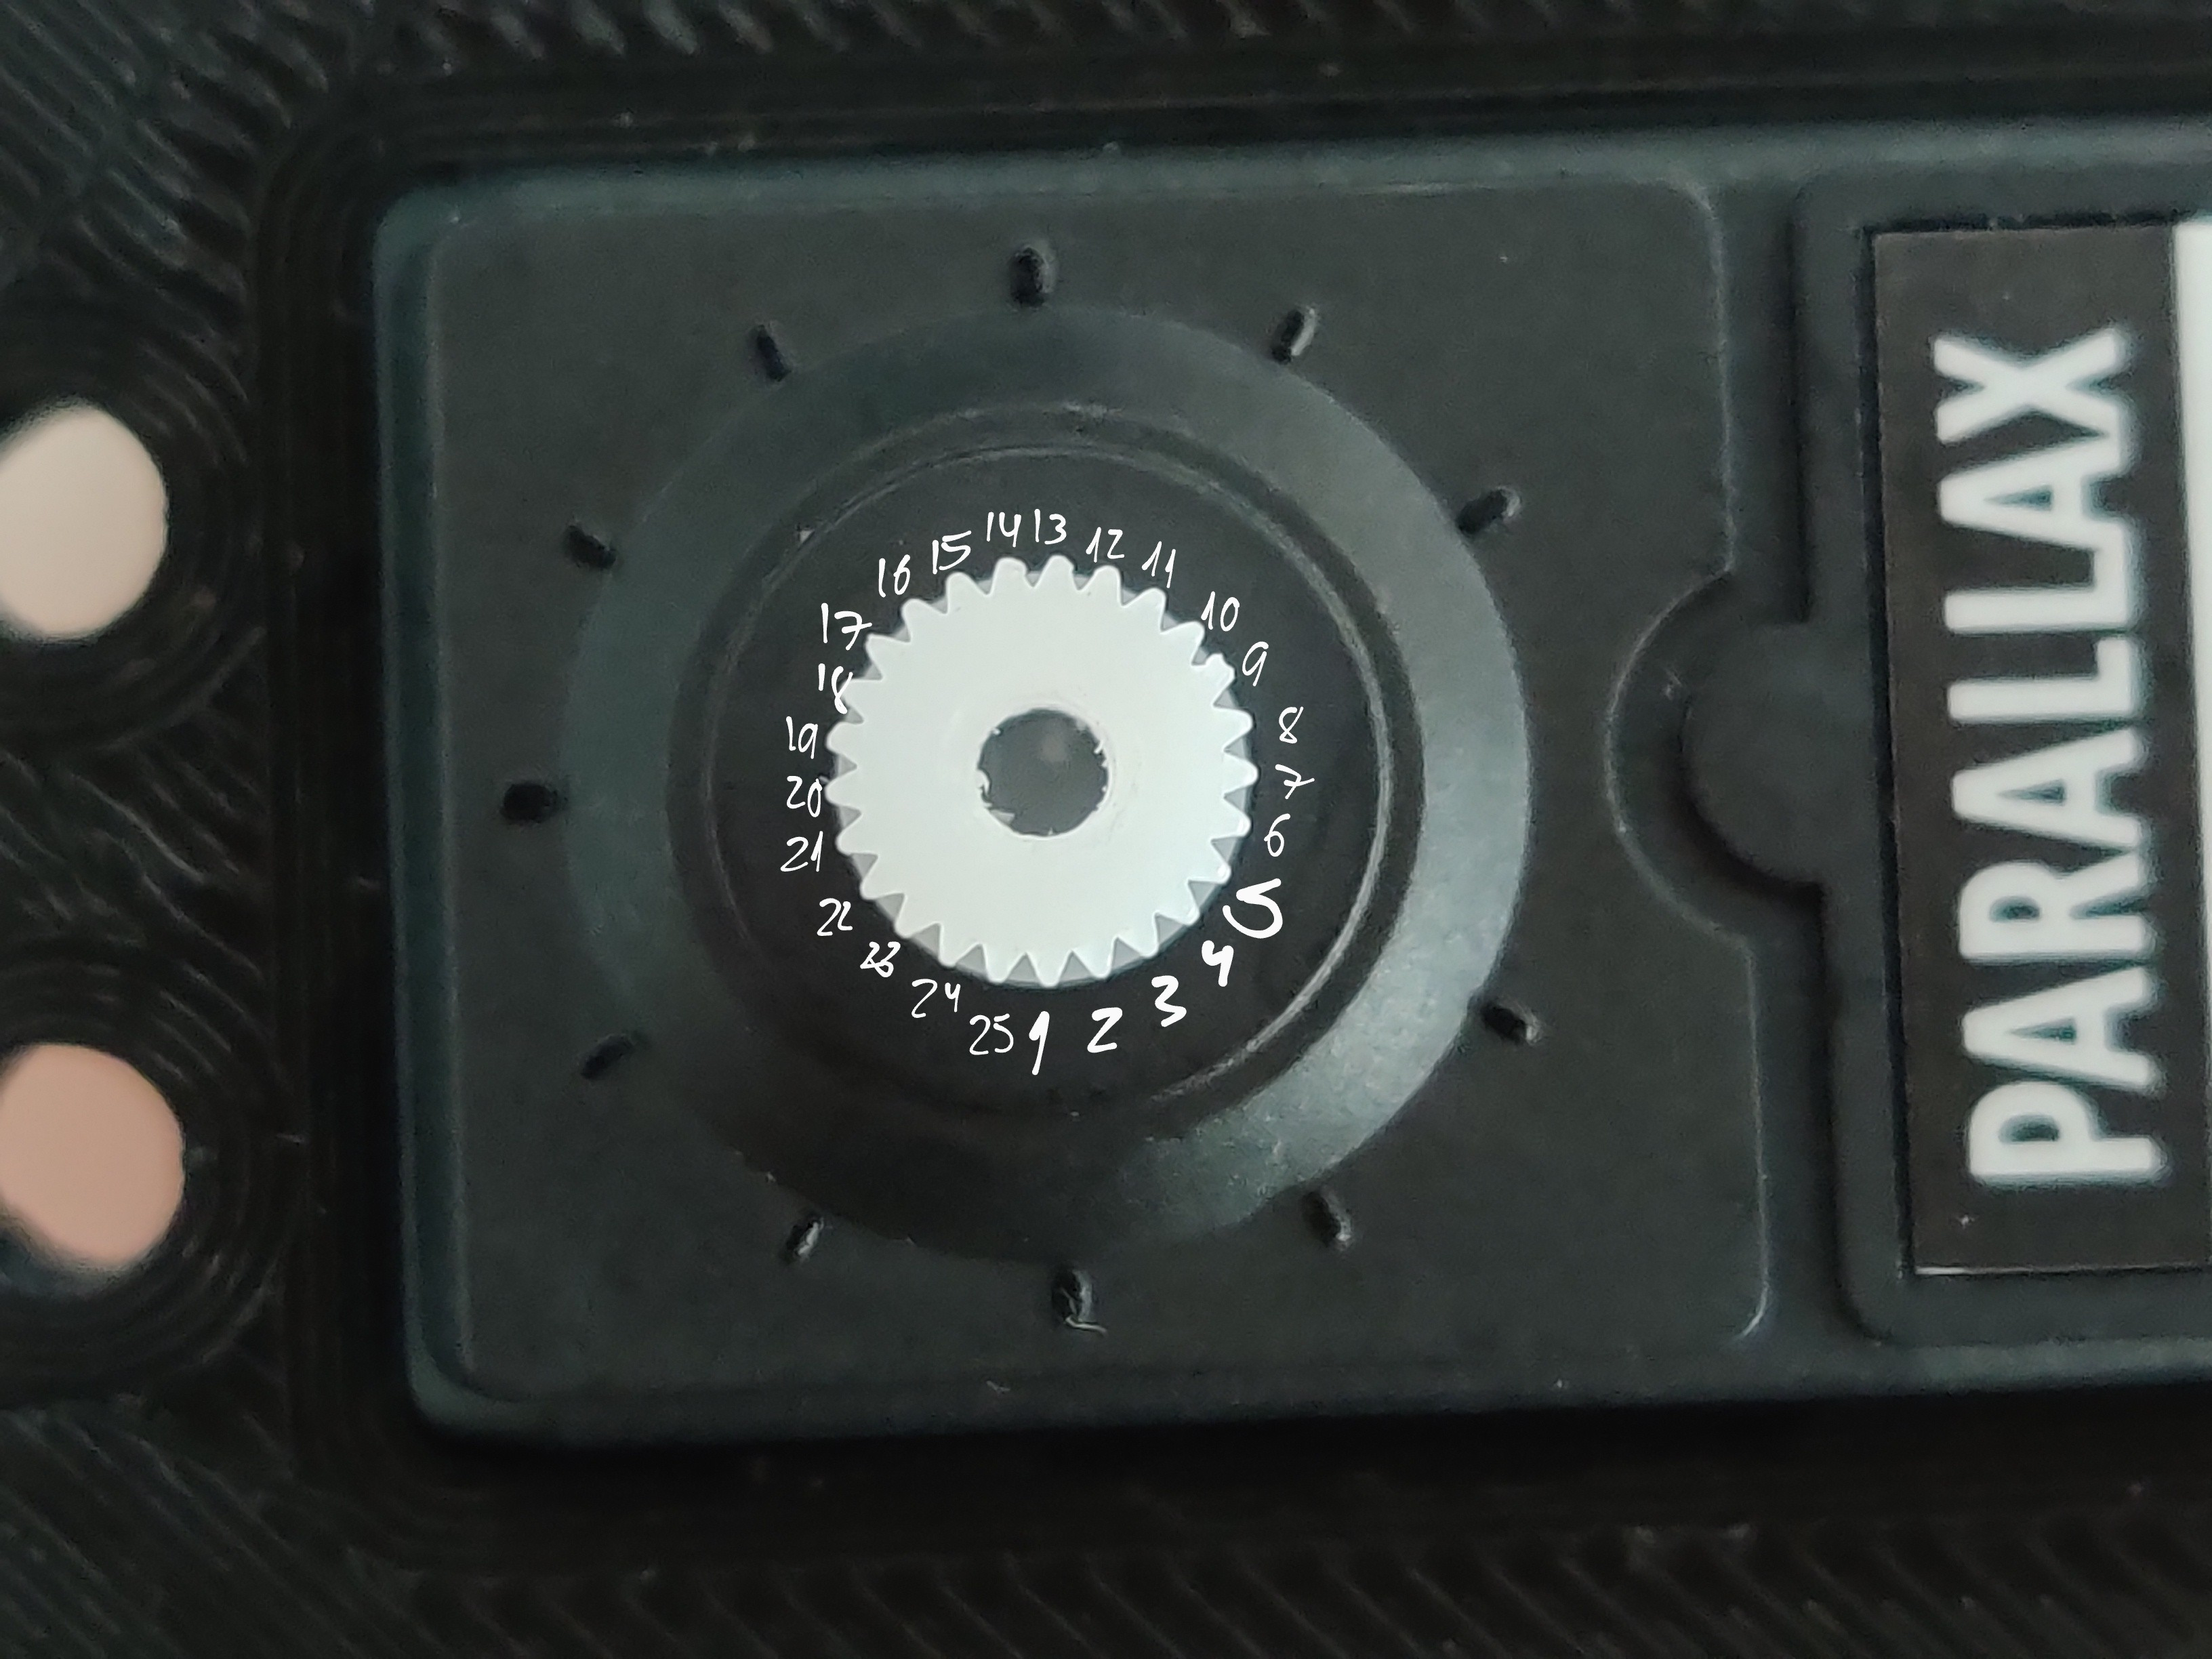
\includegraphics[width=.5\linewidth]{pictures/motor_teeth.jpg}
    \caption{Cantidad de dientes presentes en los motores empleados.}
    \label{fig:motor_teeth_count}
\end{figure}

Tras varias pruebas se concluyó que el módulo necesario 
$\left(mod = \nicefrac{\diameter}{\#dientes}\right)$ depende de si las capas que contienen 
los dientes son capas superiores o inferiores a la hora de imprimirlas.
En capas inferiores el módulo ha de ser de $\numprint[mm]{0.257}$ mientras que en
capas superiores el módulo ha de ser $\numprint[mm]{0.25}$.

Para un módulo mayor los dientes de ambos engranajes no encajaban bien y por tanto el giro no se transmitía del eje a la pieza. Para un módulo menor el eje no entraba dentro de la pieza.

Esta diferencia en el valor del módulo se debía a que las primeras capas de la impresión
3D se realizan con distinta precisión con respecto a las capas más elevadas de la
pieza, por lo que la medida ha de ser adaptada según la orientación en la que se quiera
imprimir.

\subsection{Pruebas en la impresión 3D}
Pese a que no se realizaron demasiadas pruebas propiamente dichas, destacan los siguientes
experimentos:

\begin{itemize}
    \item Se imprimió una ``seta'' para probar el soporte con \ac{PVA}, probando con
    distintas configuraciones y densidades. Esta prueba resultó satisfactoria y
    permitió avanzar en la configuración a usar para imprimir con \ac{PVA}.

    \item Se imprimieron, tal como se ha comentado en la sección anterior,
    una pieza con distintos módulos para los engranajes. Con esta prueba se descubrió
    que las primeras capas de impresión constan de menos precisión por lo que, según
    se imprima en las primeras o últimas capas, habrá que utilizar un módulo distinto.
\end{itemize}

\subsection{Pruebas post--impresión}
\label{pruebas_post_impresión}

Aprovechando ciertas piezas cuya impresión fue insatisfactoria, el equipo de desarrollo realizó pruebas destructivas para determinar el aguante ante esfuerzos de tracción, compresión y torsión.

Debido a que la estructura inferior del brazo debe soportar el peso de este, se estudió el aguante ante esfuerzos de compresión de las piezas macizas donde se concluyó que pueden aguantar pesos superiores a $\numprint[kg]{50}$ sin deformarse.

Por otro lado, el esfuerzo de tracción se ha estudiado al completar la estructura del brazo, y se ha concluido que las piezas son capaces de soportar, al menos, el propio peso de la estructura.

%El esfuerzo de torsión ha sido estudiado sobre las piezas que han de transferir el movimiento desde el eje motor hasta la estructura. También se ha concluido que será capaz de soportar al menos el propio peso de la estructura.%

Cabe destacar que en las piezas que son atravesadas por tornillos se han observado problemas en las roscas de poca profundidad. Al ser el acero un material mucho más duro que el plástico, este puede romper los surcos de las roscas si son muy superficiales, ya que el esfuerzo se realiza sobre un número más reducido de surcos que en el caso de una rosca más profunda. 
Concretamente, este problema aparece en las piezas que tienen tornillos para hacer presión sobre un eje.

Para solucionar este problema se ha decidido limar el eje en las zonas donde este entre en contacto con los tornillos, buscando conseguir una estructura cuadrada (en lugar de circular). De esta manera, la fuerza que se ha de ejercer para mantener el eje fijo es menor y por tanto no se fuerzan las roscas.